\section{PTracking}

\begin{frame}
	\frametitle{PTracking}
	
	\vspace{0.15cm}
	
	\begin{columns}[T]
		\column{.53\textwidth}
		
		\vspace{0.8cm}
		
		\begin{itemize}
			\item \textbf{Input:} a set of positions of the objects provided by a multi
				  object detection system
			
			\vspace{1.6cm}
			
			\item \textbf{Output:} a set of estimated trajectories of the moving objects
				  over time
		\end{itemize}
		
		\column{.5\textwidth}
		\centering
		
		\begin{tikzpicture}
			\node at (0,0) [draw=black,ultra thick,inner sep=0pt]
			{
				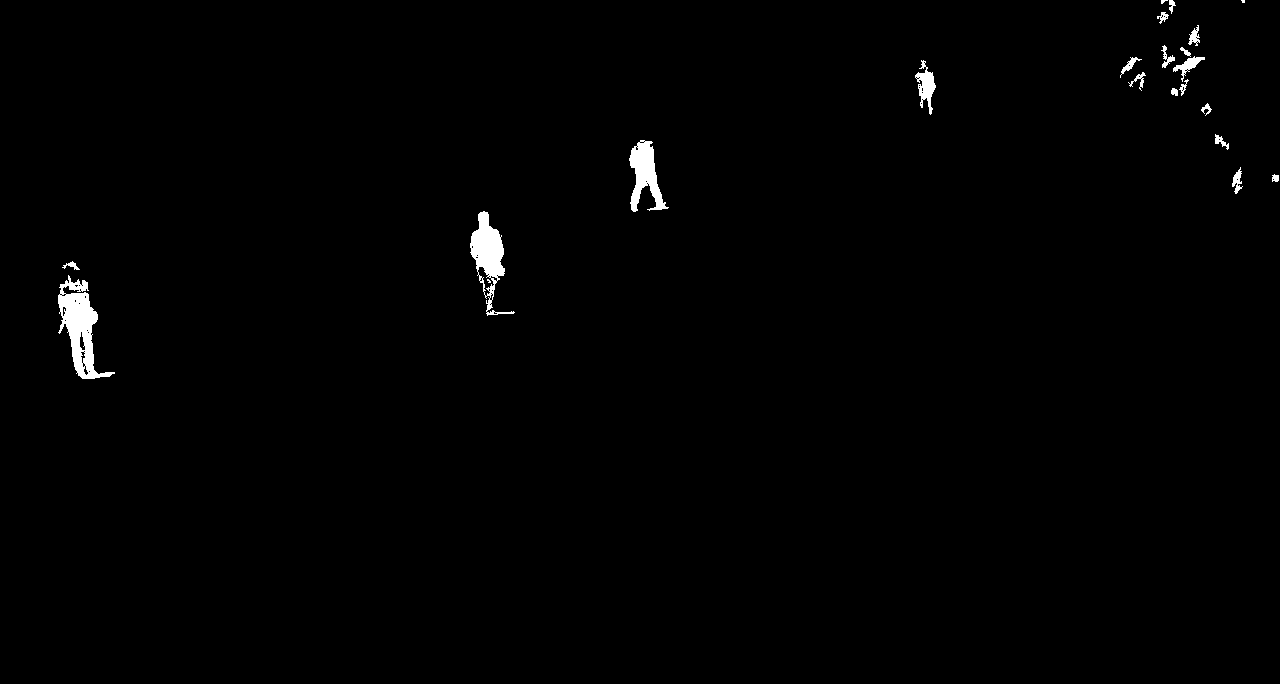
\includegraphics[width=5.8cm]{Figures/Detection}
			};
			\node at (0,-3.35) [draw=black,ultra thick,inner sep=0pt]
			{
				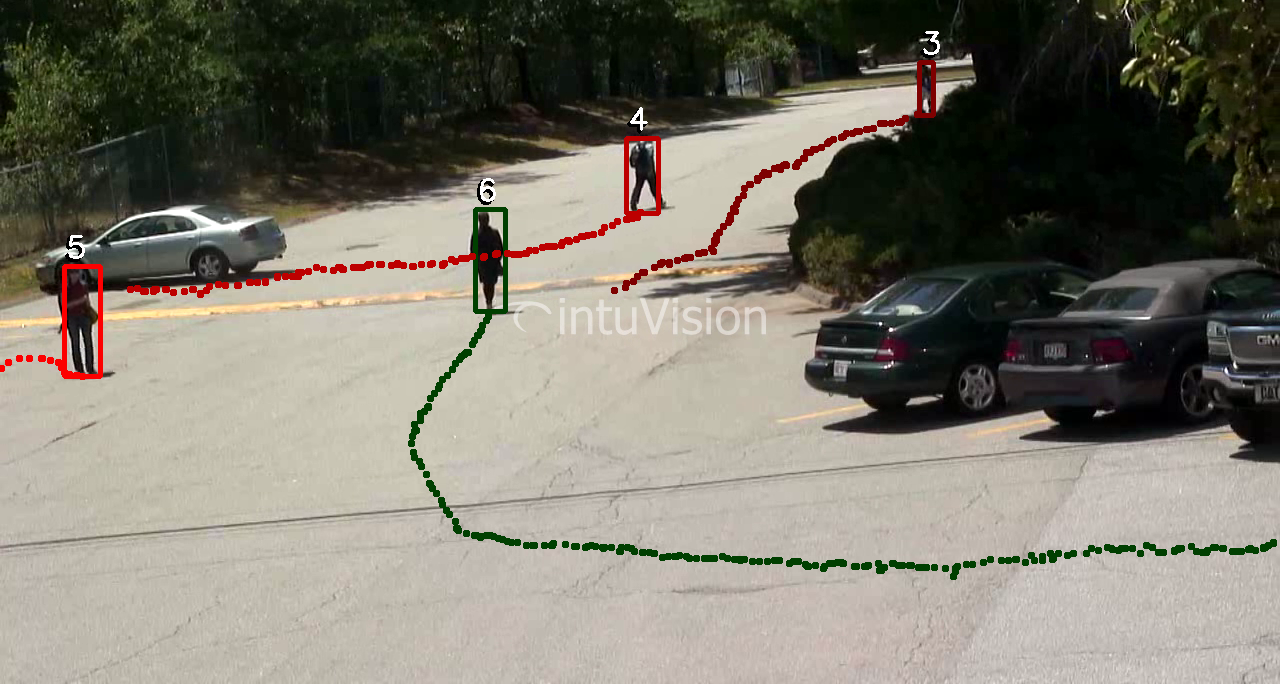
\includegraphics[width=5.8cm]{Figures/Tracking}
			};
		\end{tikzpicture}
	\end{columns}
\end{frame}

%\begin{frame}
%	\frametitle{PTracking}
%	\framesubtitle{Pseudo-code}
%	
%	\begin{columns}[T]
%		\column{.05\textwidth}
%		
%		\column{.55\textwidth}
%		
%		\only<1>
%		{
%			\begin{algorithm}[H]
%				\tiny
%				\KwIn{perceptions $ z_{s,t} $, local track numbers $ i_{s,t-1} $, global track numbers $ I_{s,t-1} $}
%				\BlankLine
%				\KwData{set of local particles $ \tilde{\xi}_{s,t} $, set of global particles $ \tilde{\xi}_{\mathcal{S'},t} $, local GMM set $ \mathcal{L} $, global GMM set $ \mathcal{G} $}
%				\BlankLine
%				\KwOut{global estimations $ x_{s,t} = (\boldsymbol{I}_{s,t},\boldsymbol\Lambda_{s,t},\boldsymbol{M}_{s,t},\boldsymbol\Sigma_{s,t}) $}
%				\BlankLine
%				\Begin
%				{
%					\textcolor{darkgreen}{$ \tilde{\xi}_{s,t} \sim \pi_t (x_{s,t} | x_{s,t-1},z_{s,t}) $}
%					\BlankLine
%					\textcolor{darkgreen}{Re-sample by using the SIR principle}\\
%					\BlankLine
%					\textcolor{darkgreen}{$ \mathcal{L} = KClusterize(\tilde{\xi}_{s,t}) $}
%					\BlankLine
%					\textcolor{darkgreen}{$ (\boldsymbol{i}_{s,t},\boldsymbol\lambda_{s,t},\boldsymbol\mu_{s,t},\boldsymbol\sigma_{s,t}) = DataAssociation(\mathcal{L}, i_{s,t-1}) $}
%					\BlankLine
%					\textcolor{darkgreen}{Communicate belief $ (\boldsymbol{i}_{s,t},\boldsymbol\lambda_{s,t},\boldsymbol\mu_{s,t},\boldsymbol\sigma_{s,t}) $ to other agents}
%				}
%				\BlankLine
%				\Begin
%				{
%					Collect $ \mathcal{L}_{S'} $ from a subset $ \mathcal{S'} \subseteq \mathcal{S} $ of sensors within a $ \Delta t $
%					\BlankLine
%					$ \tilde{\xi}_{\mathcal{S'},t} \sim \tilde\pi = \sum_{s \in \mathcal{S'}} \boldsymbol\lambda_{s,t} \, \mathcal{N} (\boldsymbol\mu_{s,t},\boldsymbol\sigma_{s,t}) $
%					\BlankLine
%					Re-sample by using the SIR principle\\
%					\BlankLine
%					$ \mathcal{G} = KClusterize(\tilde\xi_{{\mathcal{S'},t}}) $
%					\BlankLine
%					$ (\boldsymbol{I}_{s,t},\boldsymbol\Lambda_{s,t},\boldsymbol{M}_{s,t},\boldsymbol\Sigma_{s,t}) = DataAssociation(\mathcal{G},I_{s,t-1}) $
%				}
%			\end{algorithm}
%			
%			\column{.01\textwidth}
%			
%			\Huge
%			\vspace{2.15cm}
%			
%			\begin{center}
%				\textcolor{blue}{$ \Rightarrow $}
%			\end{center}
%			
%			\column{.44\textwidth}
%			
%			\centering
%			
%			\begin{tikzpicture}
%				\node at (0,0) [draw=black,ultra thick,inner sep=0pt]
%				{
%					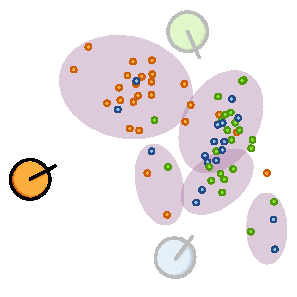
\includegraphics[width=3.3cm]{Figures/Mamot-1}
%				};
%				\node at (0,-3.5) [draw=black,ultra thick,inner sep=0pt]
%				{
%					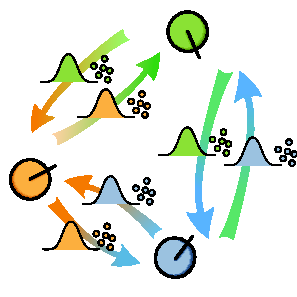
\includegraphics[width=3.3cm]{Figures/Mamot-2}
%				};
%			\end{tikzpicture}
%		}
%		
%		\only<2->
%		{
%			\begin{algorithm}[H]
%				\tiny
%				\KwIn{perceptions $ z_{s,t} $, local track numbers $ i_{s,t-1} $, global track numbers $ I_{s,t-1} $}
%				\BlankLine
%				\KwData{set of local particles $ \tilde{\xi}_{s,t} $, set of global particles $ \tilde{\xi}_{\mathcal{S'},t} $, local GMM set $ \mathcal{L} $, global GMM set $ \mathcal{G} $}
%				\BlankLine
%				\KwOut{global estimations $ x_{s,t} = (\boldsymbol{I}_{s,t},\boldsymbol\Lambda_{s,t},\boldsymbol{M}_{s,t},\boldsymbol\Sigma_{s,t}) $}
%				\BlankLine
%				\Begin
%				{
%					$ \tilde{\xi}_{s,t} \sim \pi_t (x_{s,t} | x_{s,t-1},z_{s,t}) $
%					\BlankLine
%					Re-sample by using the SIR principle\\
%					\BlankLine
%					$ \mathcal{L} = KClusterize(\tilde{\xi}_{s,t}) $
%					\BlankLine
%					$ (\boldsymbol{i}_{s,t},\boldsymbol\lambda_{s,t},\boldsymbol\mu_{s,t},\boldsymbol\sigma_{s,t}) = DataAssociation(\mathcal{L}, i_{s,t-1}) $
%					\BlankLine
%					Communicate belief $ (\boldsymbol{i}_{s,t},\boldsymbol\lambda_{s,t},\boldsymbol\mu_{s,t},\boldsymbol\sigma_{s,t}) $ to other agents
%				}
%				\BlankLine
%				\Begin
%				{
%					\textcolor{lightred}{Collect $ \mathcal{L}_{S'} $ from a subset $ \mathcal{S'} \subseteq \mathcal{S} $ of sensors within a $ \Delta t $}
%					\BlankLine
%					\textcolor{lightred}{$ \tilde{\xi}_{\mathcal{S'},t} \sim \tilde\pi = \sum_{s \in \mathcal{S'}} \boldsymbol\lambda_{s,t} \, \mathcal{N} (\boldsymbol\mu_{s,t},\boldsymbol\sigma_{s,t}) $}
%					\BlankLine
%					\textcolor{lightred}{Re-sample by using the SIR principle}\\
%					\BlankLine
%					\textcolor{lightred}{$ \mathcal{G} = KClusterize(\tilde\xi_{{\mathcal{S'},t}}) $}
%					\BlankLine
%					\textcolor{lightred}{$ (\boldsymbol{I}_{s,t},\boldsymbol\Lambda_{s,t},\boldsymbol{M}_{s,t},\boldsymbol\Sigma_{s,t}) = DataAssociation(\mathcal{G},I_{s,t-1}) $}
%				}
%			\end{algorithm}
%			
%			\column{.01\textwidth}
%			
%			\Huge
%			\vspace{2.15cm}
%			
%			\begin{center}
%				\textcolor{blue}{$ \Rightarrow $}
%			\end{center}
%			
%			\column{.44\textwidth}
%			
%			\centering
%			
%			\begin{tikzpicture}
%				\node at (0,0) [draw=black,ultra thick,inner sep=0pt]
%				{
%					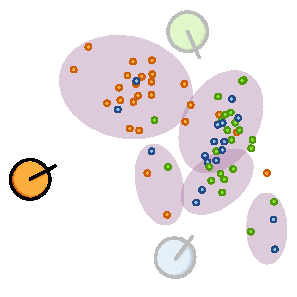
\includegraphics[width=3.3cm]{Figures/Mamot-1}
%				};
%				\node at (0,-3.5) [draw=black,ultra thick,inner sep=0pt]
%				{
%					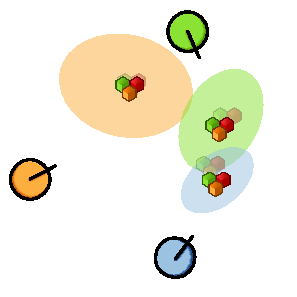
\includegraphics[width=3.3cm]{Figures/Mamot-3}
%				};
%			\end{tikzpicture}
%		}
%	\end{columns}
%\end{frame}
